\documentclass[openany]{article}

%Typesetting and language
\usepackage[american]{babel}
\usepackage[T1]{fontenc}
\usepackage{charter}
\usepackage{enumitem}
\usepackage{hyperref}

%Symbols
\usepackage{amssymb, amsmath, amsthm, bm}
\usepackage{mathrsfs}
\usepackage{mathtools}
\usepackage{marvosym}
\usepackage{MnSymbol}

%Colors & graphics
\usepackage[dvipsnames]{xcolor}
\usepackage{pgfplots}
\usepackage[numbered,framed]{matlab-prettifier}
\usepackage{pgfplots}
\usepackage{listings}
\usepackage{tikz}
\usetikzlibrary{arrows.meta}
\usepackage[object=vectorian]{pgfornament}
\usepackage{wrapfig}
\usepackage{varwidth}
\usepackage[framemethod=TikZ]{mdframed}
\usepackage{caption}
\usepackage{float}
\usepackage{geometry}
\usepackage{ulem}
\usepackage[most]{tcolorbox}
\usepackage{array}

\setlength{\parindent}{0pt}

\makeatletter
\g@addto@macro\bfseries{\boldmath}
\makeatother


\renewcommand{\Re}{\mathfrak{Re}}
\renewcommand{\Im}{\mathfrak{Im}}

\geometry{left=2cm,right=2cm,bottom=2cm,top=2cm}

\usepackage{fancyhdr}
\pagestyle{fancy}
\fancyhf{}
\renewcommand{\sectionmark}[1]{\markright{\arabic{section} - #1}}
\cfoot{\thepage}
\lhead{CS270}
\chead{HW7}
\rhead{Adam Yang}
\renewcommand{\headrulewidth}{1pt}


\DeclareMathOperator{\sgn}{sgn}
\DeclareMathOperator{\im}{im}
\DeclareMathOperator{\var}{var}
\DeclareMathOperator{\Orb}{Orb}
\DeclareMathOperator{\Fix}{Fix}
\DeclareMathOperator{\Stab}{Stab}
\DeclareMathOperator{\cov}{cov}
\DeclareMathOperator*{\esssup}{ess\,sup}
\DeclareMathOperator{\corr}{corr}
\DeclareMathOperator{\lik}{lik}
\DeclareMathOperator*{\argmin}{argmin}
\DeclareMathOperator*{\argmax}{argmax}

\newcommand{\niceline}[2]{%
		\nointerlineskip \vspace{.5\baselineskip}\hspace{\fill}
		{\color{#1}
				\resizebox{0.5\linewidth}{2ex}
				{{%
								{\begin{tikzpicture}
										\node  (C) at (0,0) {};
										\node (D) at (9,0) {};
										\path (C) to [ornament=#2] (D);
										\end{tikzpicture}}}}}%
		\hspace{\fill}
		\par\nointerlineskip \vspace{.5\baselineskip}
}

\definecolor{darkViolet}{HTML}{9400D3}
\newcommand{\sweetline}{%
		\noindent
		\begin{center}
				{\color{darkViolet}
						\resizebox{0.5\linewidth}{1ex}
						{{%
										{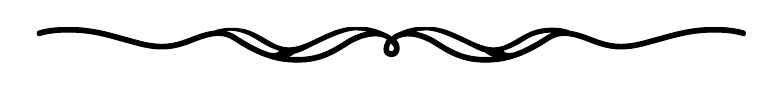
\begin{tikzpicture}
												\node  (C) at (0,0) {};
												\node (D) at (9,0) {};
												\path (C) to [ornament=85] (D);
												\end{tikzpicture}}}}}%
		\end{center}
}

\definecolor{remarkPurple}{HTML}{8346FF}
\definecolor{defBlue}{HTML}{0673FF}
\definecolor{exPurple}{HTML}{FF8710}

%THEOREM
\newtcbtheorem[auto counter,number within=section]{theorem}{Theorem}%
{enhanced,colback=white, breakable,frame empty,interior empty,colframe=cyan!50!white, top=8mm,
				coltitle=black,fonttitle=\bfseries,colbacktitle=cyan!15!white,
				borderline={0.5mm}{0mm}{cyan!15!white},
				borderline={0.5mm}{0mm}{cyan!50!white,dashed},
				attach boxed title to top left={yshift=-4mm},
				boxed title style={sharp corners=east,boxrule=1pt},varwidth boxed title}{thm}

%PROPOSITION
\newtcbtheorem[use counter from=theorem]{proposition}{Proposition}%
{enhanced,colback=white,breakable,frame empty,interior empty,colframe=defBlue!75!white, top=8mm,
				coltitle=black,fonttitle=\bfseries,colbacktitle=defBlue!20!white,
				borderline={0.5mm}{0mm}{defBlue!20!white},
				borderline={0.5mm}{0mm}{defBlue!50!white,dashed},
				attach boxed title to top left={yshift=-4mm},
				boxed title style={sharp corners=east,boxrule=1pt},varwidth boxed title}{prop}

%DEFINITION
\newtcbtheorem[use counter from=theorem]{definition}{Definition}%
{enhanced,colback=white,breakable,frame empty,interior empty,colframe=defBlue!75!white, top=8mm,
				coltitle=black,fonttitle=\bfseries,colbacktitle=defBlue!20!white,
				borderline={0.5mm}{0mm}{defBlue!20!white},
				borderline={0.5mm}{0mm}{defBlue!50!white,dashed},
				attach boxed title to top left={yshift=-4mm},
				boxed title style={sharp corners=east,boxrule=1pt},varwidth boxed title}{def}

%COROLLARY
\newtcbtheorem[use counter from=theorem]{corollary}{Corollary}%
{enhanced,colback=white,breakable,frame empty,interior empty,colframe=defBlue!75!white, top=8mm,
				coltitle=black,fonttitle=\bfseries,colbacktitle=defBlue!20!white,
				borderline={0.5mm}{0mm}{defBlue!20!white},
				borderline={0.5mm}{0mm}{defBlue!50!white,dashed},
				attach boxed title to top left={yshift=-4mm},
				boxed title style={sharp corners=east,boxrule=1pt},varwidth boxed title}{cor}

%REMARK
\newtcbtheorem[no counter]{remark}{Remark}%
{detach title, colback=white,enhanced ,breakable,frame empty, interior empty, fonttitle=\bfseries, coltitle=Violet, before upper={\tcbtitle.\quad},
				borderline west={0.5mm}{0mm}{remarkPurple!40!white},
				borderline west={0.5mm}{0mm}{remarkPurple!60!white,dashed}}{remark}

%LEMMA
\makeatletter
\newtcbtheorem[number within = tcb@cnt@theorem]{lemma}{Lemma}%
{enhanced,breakable,colback=white,frame empty,interior empty,colframe=orange!75!white, top=8mm,
				coltitle=black,fonttitle=\bfseries,colbacktitle=orange!20!white,
				borderline={0.5mm}{0mm}{orange!20!white},
				borderline={0.5mm}{0mm}{orange!50!white,dashed},
				attach boxed title to top left={yshift=-4mm},
				boxed title style={sharp corners=east,boxrule=1pt},varwidth boxed title}{lemma}
\makeatother


%PROOF
%%{enhanced,breakable,frame empty,interior empty,colframe=remarkPurple!75!white, top=8mm,
%	coltitle=black,fonttitle=\bfseries,colbacktitle=remarkPurple!20!white,
%	borderline={0.5mm}{0mm}{remarkPurple!20!white},
%	borderline={0.5mm}{0mm}{remarkPurple!50!white,dashed},
%	attach boxed title to top left={yshift=-4mm},
%	boxed title style={sharp corners=east,boxrule=1pt},varwidth boxed title}{prf}


\tcolorboxenvironment{proof}{% amsthm' 
				blanker,breakable,left=5mm,
				before skip=10pt,after skip=10pt,
				borderline west={0.5mm}{0pt}{cyan!40},
				borderline west={0.5mm}{0pt}{remarkPurple!10, dashed}}

%PROBLEM
\newtcbtheorem[auto counter]{problem}{Problem}%
{enhanced,breakable,colback=white,frame empty,interior empty,colframe=cyan!50!white, top=8mm,
				coltitle=black,fonttitle=\bfseries,colbacktitle=cyan!20!white,
				borderline={0.5mm}{0mm}{cyan!20!white},
				borderline={0.5mm}{0mm}{cyan!50!white,dashed},
				attach boxed title to top left={yshift=-4mm},
				boxed title style={sharp corners=east,boxrule=1pt},varwidth boxed title}{prob}

%EXAMPLE
%\newtcbtheorem[use counter from=problem]{example}{Example}%
%{enhanced,breakable,colback=white,frame empty,interior empty,colframe=remarkPurple!50!white, top=8mm,
%		coltitle=black,fonttitle=\bfseries,colbacktitle=remarkPurple!30!white,
%		borderline={0.5mm}{0mm}{remarkPurple!30!white},
%		borderline={0.5mm}{0mm}{remarkPurple!30!white,dashed},
%		attach boxed title to top left={yshift=-4mm},
%		boxed title style={sharp corners=east,boxrule=1pt},varwidth boxed title}{ex}


\newtcbtheorem[use counter from=theorem]{example}{Example}%
{detach title, colback=white,enhanced ,breakable,frame empty, interior empty, fonttitle=\bfseries, coltitle=black, before upper={\tcbtitle.\quad},
		borderline west={0.5mm}{0mm}{remarkPurple!30!white},
		borderline ={0.5mm}{0mm}{remarkPurple!30!white}}{example}

%SOLUTION
\newtcbtheorem[no counter]{solution}{Solution}%
{enhanced,breakable,colback=white,frame empty,interior empty,colframe=green!75!white, top=8mm,
				coltitle=black,fonttitle=\bfseries,colbacktitle=green!20!white,
				borderline={0.5mm}{0mm}{green!20!white},
				borderline={0.5mm}{0mm}{green!50!white,dashed},
				attach boxed title to top left={yshift=-4mm},
				boxed title style={sharp corners=east,boxrule=1pt},varwidth boxed title}{sol}
\definecolor{realPurple}{HTML}{AA05F9}
\definecolor{gray}{rgb}{0.5,0.5,0.5}
\definecolor{dkgreen}{rgb}{0,0.6,0}
\definecolor{mauve}{rgb}{0.58,0,0.82}

\lstset{frame=tb,
				style=Matlab-editor,
				language=C,
				aboveskip=3mm,
				belowskip=3mm,
				xleftmargin=3mm,
				showstringspaces=false,
				columns=flexible,
				frame=none,
				basicstyle={\small\ttfamily},
				numberstyle=\tiny\color{gray},
				keywordstyle=\color{blue},
				commentstyle=\color{dkgreen},
				stringstyle=\color{mauve},
				breaklines=true,
				breakatwhitespace=true,
				mlshowsectionrules = true,
				tabsize=3,
                    escapechar = ~,
				backgroundcolor=\color{cyan!5}
}

\newcommand\mmybox[2][fill=cyan!20]{%
    \tikz[baseline]\node[%
        inner ysep=0pt, 
        inner xsep=2pt, 
        anchor=text, 
        rectangle, 
        rounded corners=1mm,
        #1] {\strut#2};%
}


\def\changemargin#1#2{\list{}{\rightmargin#2\leftmargin#1}\item[]}
\let\endchangemargin=\endlist

\linespread{1.4}



% MAIN DOC
\begin{document}

\title{HW 7}
\author{Adam Yang}
% \date{\today}
\maketitle




\section*{Problem1}

In Problem 1, we are given a graph $G=(V,E)$, each node $e\in E$ has non-negative capacities $c_e$, a source node $s$ which has no edge flows into, and a sink node $t$ which has no edge flows out, and a flow $f$ and value $\nu(f)$.

\subsection*{Algorithm}
\begin{proof}[Algorithm]{}
		\renewcommand{\qedsymbol}{}
		An Algorithm to output a new flow $f'$ with $f'_e \leq f_e$ for all edges $e$, of the same value $\nu(f') = \nu(f)$, and such that $f'$ is acyclic.
		\begin{lstlisting}[basicstyle=\fontsize{8}{9}\selectfont\ttfamily]
~$f':=$~ the new flow that we will output
~$f' = f$~ at the beginning
while ~$G$~ contains a cycle:
    do BFS to find a cycle ~$C$~ in ~$G$~
    define any cycle found as ~$C \subseteq E_{exists}$~:
        let ~$\varepsilon = \mathbf{\min}(f(e))$~, ~$\forall e\in C$~
        subtract ~$\varepsilon$~ from the flow of all edge in ~$C$~ on instance ~$f'$~
        ~$\forall e$~ in ~$C:$~ ~$f'(e)=0$~, delete e from the graph

return new flow ~$f'$~
		\end{lstlisting} 
\end{proof}

\textbf{Observations:}

1. source node $s$ and sank node $t$ cannot be involved in any cycle because they all only have one-way edges.

2. $f$ is a valid flow that satisfies Conservation, Capacity, Non-negativity properties

\subsection*{Proof}
\begin{proof}[1]{To prove that $f'$ is a valid flow}
(a) Conservation

Focus on a cycle $C \subseteq E_{exists}$, $C$ has a set of node $\{v_1, v_2, ..., v_k\}, 1 < k \leq n$. Define the $e_{i,in} \in C$ for $v_i$ as the in-flow edge, $e_{i,out} \in C$ as the out-flow edge in the cycle. Define $s_{i,in} \notin C$ as the in-flow edge for $v_i$ that is not in cycle and $s_{i,out} \notin C$ as the out-flow edge for $v_i$ that is not in cycle. Define $f_{in}(v_i)$ and $f_{out}(v_i)$ as the total in-flow and out-flow for $v_i$.

In the algorithm, we find smallest flow $\varepsilon$ from all the $f(e), e\in C$ and then subtract all edge in $C$ with $\varepsilon$.

Before subtraction, \[\forall v_i \in \{v_1, ..., v_k\}: f_{in}(v_i) = f(e_{i,in}) + \sum_{s_{i,in}} f(s_{i,in}) = f_{out}(v_i) = f(e_{i,out})+\sum_{s_{i,out}} f(s_{i,out}) \]

Since the assignment in algorithm doesn't impact the edge not in cycle, therefore $\sum_{s_{i,in}} f(s_{i,in}) = \sum_{s_{i,out}} f(s_{i,out})$. Therefore, the in-flow and out-flow doesn't change for $v_i$:

\[f_{in}(v_i) - \varepsilon = f(e_{in} \in C) + \sum_{s_{i,in}} f(s_{i,in}) - \varepsilon = f(e_{out} \in C) \sum_{s_{i,out}} f(s_{i,out}) - \varepsilon = f_{out}(v_i) - \varepsilon\]

Therefore, every node in $C$ is still conservative. for all nodes that are included cycle, conservation holds.


\end{proof}

\begin{proof}[2]{To prove capacity doesn't exceed}
    \[f'(e) = f(e) - \varepsilon \leq f(e) \leq c(e)\] because $f$ is a valid flow
    
\end{proof}

\begin{proof}[3]{To prove each flow is non-negative}
    \[f'(e) = f(e) - \varepsilon \geq 0\] because $\varepsilon = \mathbf{\min}(f(e))$ and thus $\varepsilon \leq f(e)$, $\forall e \in C$
    
\end{proof}

Therefore, $f'$ is a valid flow. Since $s$ and $t$ are not included in any cycle, the sum of out-flow for $s$ doesn't change since no subtraction happens on these edges. Similarly, the sum of in-flow for $t$ doesn't change. Also, as conservation holds for all nodes included in cycles.
\[\nu(f') = \nu(f)\]

\begin{proof}[4]{To the algorithm terminates and output an acyclic graph}

Because in each iteration, we strictly "delete" at least an edge to remove a cycle. Meanwhile, $G$ only has finite amount of cycle. Therefore, we at most delete all the edge in the graph and will finally remove all the cycle, which leads to the end of termination.
    
\end{proof}

\subsection*{Running Time}
Define $|E| = m$, $|V| = n$.

Notice that we at least delete one edge to remove one cycle in each iteration, and we only have finite amount of cycles in $G$, the iteration at most repeats $\mathcal{O}(m)$ times. 

\section*{Problem2}
In Problem 2, $m$ denotes the number of drivers, $n$ denotes the number of consumers. For each consumer $i$, we have their location $L_i$, the location of 
\subsection*{Algorithm}
\begin{proof}[Algorithm]{}
		\renewcommand{\qedsymbol}{}
		An Algorithm to ...
		\begin{lstlisting}[basicstyle=\fontsize{8}{9}\selectfont\ttfamily]


        
		\end{lstlisting} 
\end{proof}

\subsection*{Proof}
\begin{proof}[Correctness]{}

\end{proof}

\subsection*{Running Time}


\end{document}
